%! TEX root = ../main.tex
\documentclass[../main.tex]{subfiles}
\begin{document}
\section{Kapazitäten und Grenzen der Maschinen}
\subsection{Verwendbare Materialien}
Im Rahmen des \acrlong{slm}-Prozesses sind viele Materialien verarbeitbar, darunter Werkzeugstähle, Edelstähle, Titanium-Legierungen und Nickel-Legierungen. Jedes dieser Materialen findet andere Anwendungen, einige von welchen in Unterpunkt \ref{sec:anwendungen} genauer erläutert werden.\\ Tabelle \ref{table:materials} zeigt eine Übersicht der wichtigsten Materialien und deren Anwendungen. Die meisten dieser Materialien sind sowohl im \acrshort{slm} als auch im \acrshort{lmd}-Verfahren verwendbar, wenn auch teilweise in anderen Formen, wie Draht und Pulver.
\begin{table}[H]
\begin{tabularx}{\textwidth}{{>{\hsize=.6\hsize\linewidth=\hsize}X
>{\hsize=1.4\hsize\linewidth=\hsize}X}}
	\hline
	Eisen-Legierungen/Stähle & Werkzeuge (Gussformen) für Spritzguss-Verfahren, Schneidewerkzeuge, korrosive Umgebungen\\
	\hline
	Titan-Legieriungen & Medizinische Implantate (siehe Unterpunkt \ref{sec:medizin}) \\
	\hline
	Nickel-Legierungen & Hoch-Temperatur-Anwendungen (Triebwerke, Reaktoren, o.Ä.)\\
	\hline
	Kupfer-Legierungen & Elektroden, Werkzeuge, o.Ä.\\
	\hline 
	Cobalt-Legierungen & Medizinische Anwendungen, Hoch-Temperatur-Anwendungen \\
	\hline
	Aluminium-Legierungen & Anwendungen mit geringen Gewichtsanforderungen, Hitzeleitfähigkeit\\
	\hline
\end{tabularx}
\label{table:materials}
\caption{Materialien, welche im Metall-3D-Druck verwendet werden und ihre Anwendungen. \protect\parencite{nickel_1}}
\end{table}
\subsection{Geschwindigkeit}
\subsubsection*{Selective Laser Melting}
Im \acrshort{slm}-Verfahren ist die Geschwindigkeit oft durch die benötigte Hitze, die der Laser an einer Stelle liefern muss, um das Material dort aufzuschmelzen limitiert. Stärkere Laser erlauben theoretisch höhere Geschwindigkeiten, sind jedoch in der Realität unleistbar. Die meisten Drucker können aus diesem Grund mit verschiedenen Laser-Konfigurationen ausgestattet werden. Beispielsweise ist es mit einem \it{EOS M400 Series} möglich, einen einzigen \qty{1}{\kilo\watt} Laser zu erhalten für Materialien mit höherem Schmelzpunkt, oder vier \qty{400}{\watt} Laser für gleichzeitiges Drucken mehrerer einzelner Teile oder der Beschleunigung des Druckes von einem Teil, wobei dabei eher Materialien mit niedrigerem Schmelzpunkt verwendet werdenaufgrund des verringerten Energie-Outputs von jedem der einzelnen Laser.\parencite{eosm400,eosm400_4}
\subsubsection*{Laser Metal Deposition}
Im \acrlong{lmd}-Prozess sind die Möglichkeiten, die Produktionsgeschwindigkeit zu erhöhen stark begrenzt durch den Fakt, dass in den meisten Maschinen nur eine Düse einsetzbar ist. Es ist dennoch möglich, durch Düsen mit größerem Material-Durchlass eine höhere Druckgeschwindigkeit zu erreicht, wobei dabei feine Strukturen schwerer druckbar werden. Die genauen Einstellungen und Kapazitäten sind von Maschine zu Maschine unterschiedlich und hängen von viel mehr Faktoren ab als im \acrlong{slm}, darunter der genaue Aufbau des Bauteils und das verwendete Material. \parencite{Mahamood2017}
\subsection{Recycling des Exzess-Materials}
Recycling des Restmaterials ist nur bei \acrshort{slm} von Bedeutung, da bei \acrshort{lmd} kein Restabfall entsteht. Im \acrshort{slm} ist mit Restmaterial das Pulver, welches sich nach Fertigstellung des Bauteils noch im Bett rundherum befindet gemeint. Dieses ist mit kleinen Spritzern durchzogen, welche aus der Schmelze des Lasers entsprungen sind. Da diese um einige Größenordnungen über dem Durchmesser des Pulvers liegen, sind diese höchst problematisch und können das Wiederbeschichtungswerkzeug beschädigen beim nächsten Durchlauf. Deswegen werden viele der \acrshort{slm}-Maschine entweder mit einer eingebauten Siebestation geliefert oder es wird eine externe angeboten. Diese haben zumeist eine Maschenweite von \qty{50}{\micro\meter}-\qty{80}{\micro\meter} und filtern somit jegliche Partikel aus, welche dem Prozess schaden könnten. Oft vibrieren diese Siebe mit einer hohen Frequenz, um das Material effektiver und schneller zu reinigen. Dadurch ist theoretisch eine \qty{100}{\percent}ige Materialeffizienz möglich. 
\subsection{Auswirkungen von Orientierung und Platzierung}
Im Selective-Laser-Melting-Verfahren ist die richtige Orientierung im Slicer essentiell, um stabile Teile zu erhalten.
Ein Winkel von \qty{45}{\degree} führt zu einem Teil, welcher in alle Richtungen die universell größtmögliche Stärke aufweisst. Dies wird in Abb. \ref{img:ss_1} für einen Teil welcher dem Stressprofil von Abb. \ref{img:fh_1} folgt dargestellt. 
\begin{figure}[H]
	\centering
	\includegraphics[width=0.5\textwidth]{ss_Flachstab}
	\ccaption{Modell mit generierten Supports in Magics Materialise 25.02}{eigener Screenshot}
	\label{img:ss_1}
\end{figure}
\begin{figure}[H]
	\centering
	\includegraphics[width=0.5\textwidth]{fh_Flachstab}
	\ccaption{Simuliertes Lastenprofil für ein Teil mit bestimmten Verschraubungen und gleichmäßiger Last}{Screenshot Studentenaufgabe FH Wels: Ing. Walter Kaindl}
	\label{img:fh_1}
\end{figure}

Wenn ein anderes Stressprofil bekannt ist, kann mithilfe der Orientierung auch auf dieses eingegegangen werden. Allgemein sollte immer entgegen der Schichten gleichmäßig Last ausgeübt werden, da die Schicht-zu-Schicht-Verbindung der schwächste Punkt ist und beidseitige/biegende Last normal zu den Schichten wie in Abb. \ref{img:orient_1} erkennbar ist.

\begin{figure}[H]
	\centering
	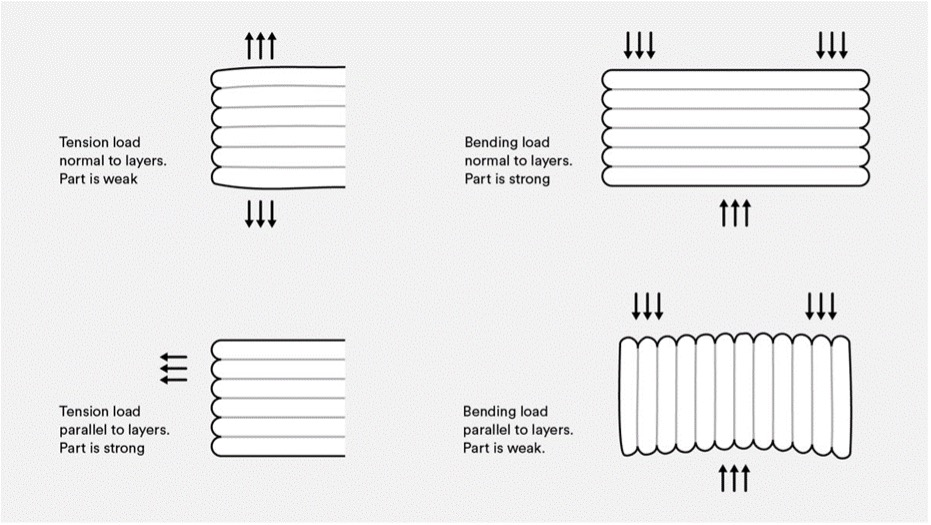
\includegraphics[width=0.8\textwidth]{orientation}
	\ccaption{Optimale Orientierung nach Lastenprofil}{https://www.protolabs.com/media/if4besvl/picture1.jpg}
	\label{img:orient_1}
\end{figure}
Zusätzlich ist die Orientierung auch bei der Platzierung der Supportstrukturen am Bauteil wichtig, da durch strategisches Rotieren des Teils die Supports minimiert werden können (Überhänge welche nicht unterstützt werden müssen o.Ä.) und somit auch Material und \it{Post-Processing}-Arbeit eingespart werden können. 

\begin{figure}[H]
	\centering
	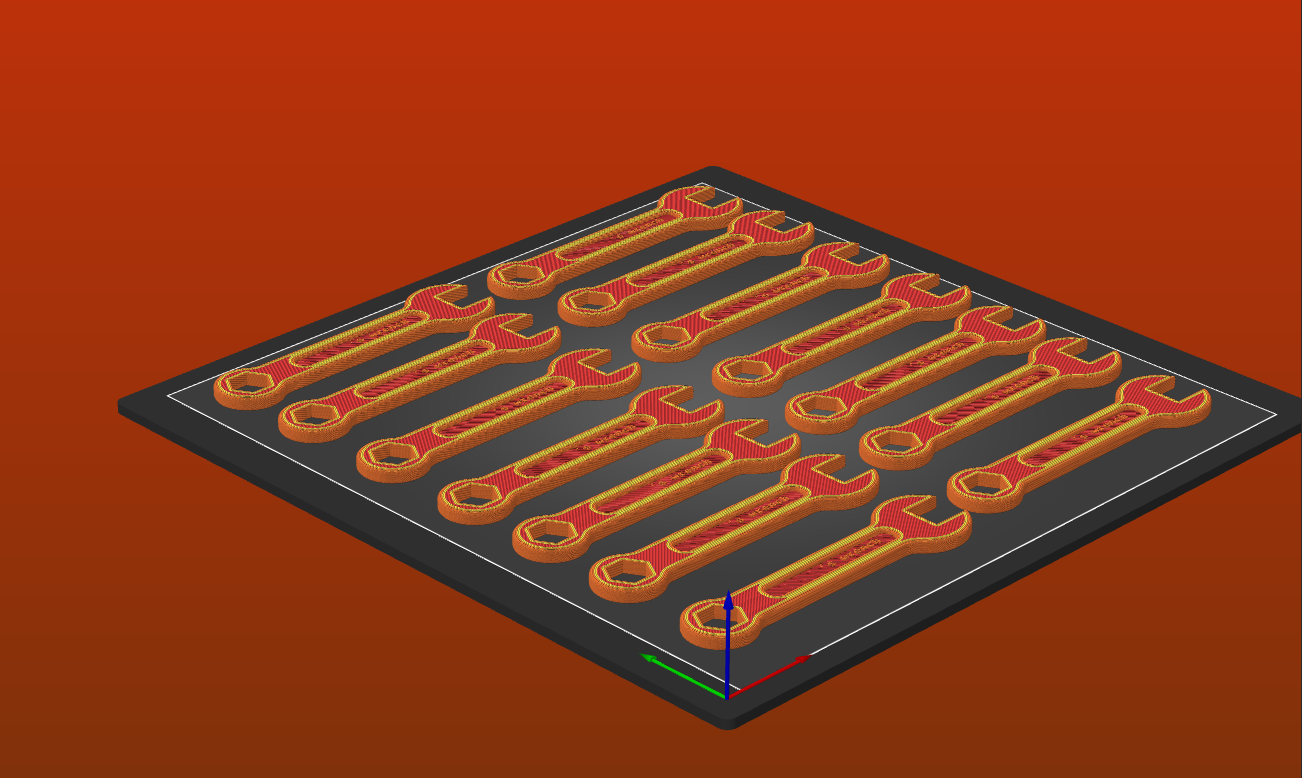
\includegraphics[width=0.5\textwidth]{unsupported}
	\ccaption{Geschwindigkeitsoptimierter Druck}{Eigener Screenshot PrusaSlicer 2.6.0}
	\label{img:unsupp_1}
\end{figure}
\begin{figure}[H]
	\centering
	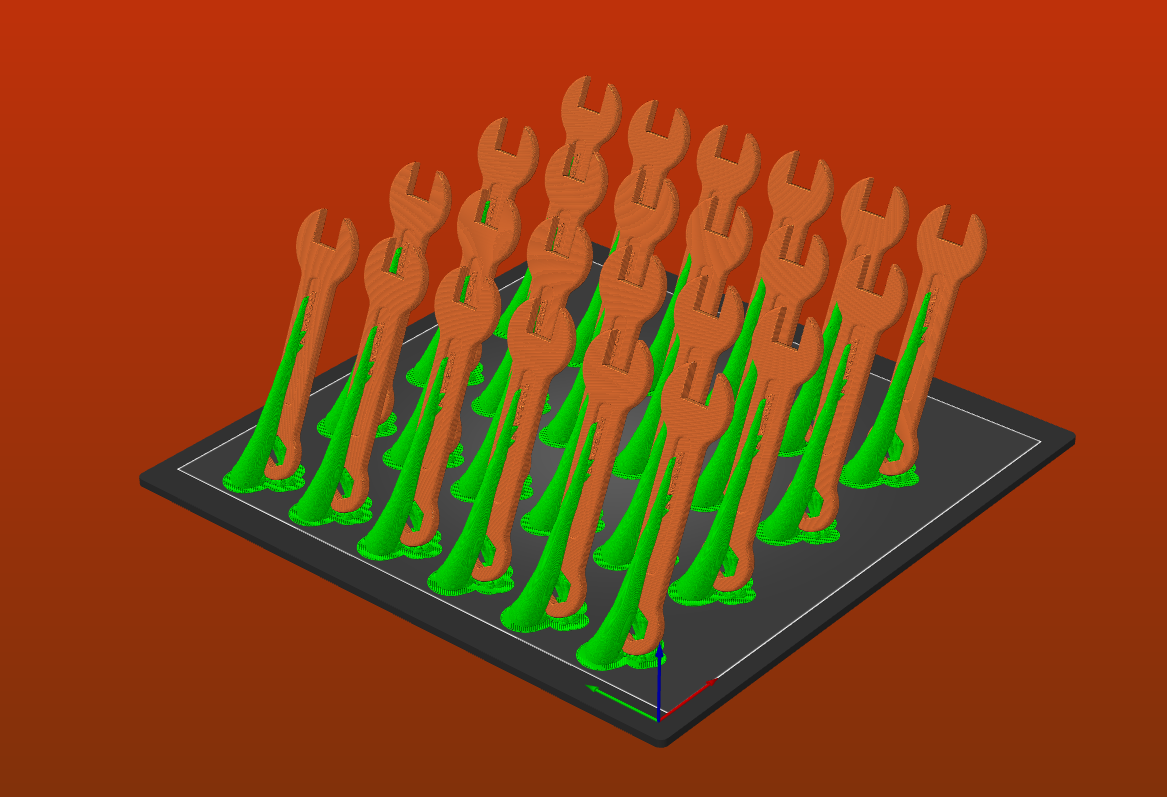
\includegraphics[width=0.5\textwidth]{supported}
	\ccaption{Massenproduktionsoptimierter Druck}{Eigener Screenshot PrusaSlicer 2.6.0}
	\label{img:supp_1}
\end{figure}
In der Massenproduktion wird zusätzlich dazu auch noch versucht, den Teil so hoch wie nur möglich zu orientieren, um den Platzverbrauch auf der Bauplatte zu minimieren wie in Abb. \ref{img:unsupp_1} und Abb. \ref{img:supp_1} zu erkennen ist. Durch diese Optimierung konnte die Produktionszahl in einem Druckvorgang beinahe verdoppelt werden.  zu erkennen ist. Durch diese Optimierung konnte die Produktionszahl in einem Druckvorgang beinahe verdoppelt werden.  zu erkennen ist. Durch diese Optimierung konnte die Produktionszahl in einem Druckvorgang beinahe verdoppelt werden.  zu erkennen ist. Durch diese Optimierung konnte die Produktionszahl in einem Druckvorgang beinahe verdoppelt werden. Der dabei entstehende Zeitaufwand durch das Drucken der Supportstrukturen ist dabei kein Nachteil, da diese Prozesse unbeaufsichtigt über Nacht laufen können und so die höhere Stückzahl am nächsten Arbeitstag dennoch fertig ist. \cite{lim2015}

Bei \acrfull{lmd} kommt hierzu noch der Fakt, dass die die Maschine zumeist nicht darauf angewiesen ist Schicht für Schicht aufzubauen, sondern es auch möglich ist damit von der Seite Objekt aufzutragen wie in Abb. \ref{img:t_pipe} erkennbar ist. Dort wird wie üblich der gelbe Teil von unten nach oben schichtweise gedruckt, und für den roten Teil rotiert der Druck-Kopf um \qty{90}{\degree}, um damit die Supportstrukturen einzusparen. Zudem ist es im \acrshort{lmd} auch möglich, dadurch ein Teil für verschiendene Last-Profile gleichzeitig zu optimieren und schönere Oberflächen zu erhalten ohne Nachbearbeitung wie in Abb. \ref{img:orient_1} erkenntlich ist. Wenn die runde Oberfläche parallel zur Bauplatte ist werden dort die Schichtlinien sehr stark und auffällig. Steht sie jedoch normal dazu sind nur gleichmäßige Schichtlinien normal zur Oberfläche erkennbar, welche schneller entfernt sind und akkuratere Dimensionen einhalten können.
\begin{figure}[H]
	\centering
	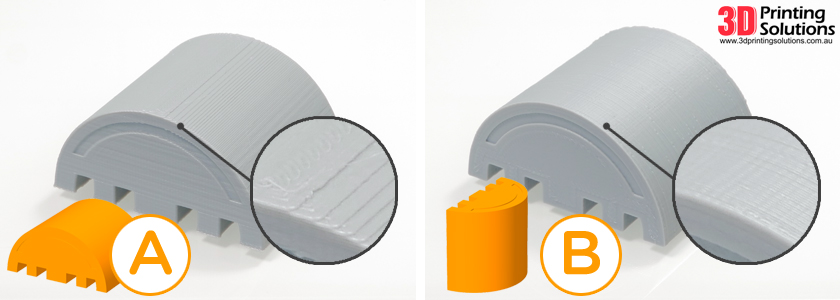
\includegraphics[width=0.5\textwidth]{round_orientation}
	\ccaption{Auswirkung von Orientierung auf runde Oberflächen}{\url{https://www.3dprintingsolutions.com.au/Portals/1/EasyGalleryImages/1/1169/HowToPrint-Model-Orientation-Quality-Circle-Layers.jpg}}

	\label{img:round_orient}
\end{figure}
\begin{figure}[H]
	\centering
	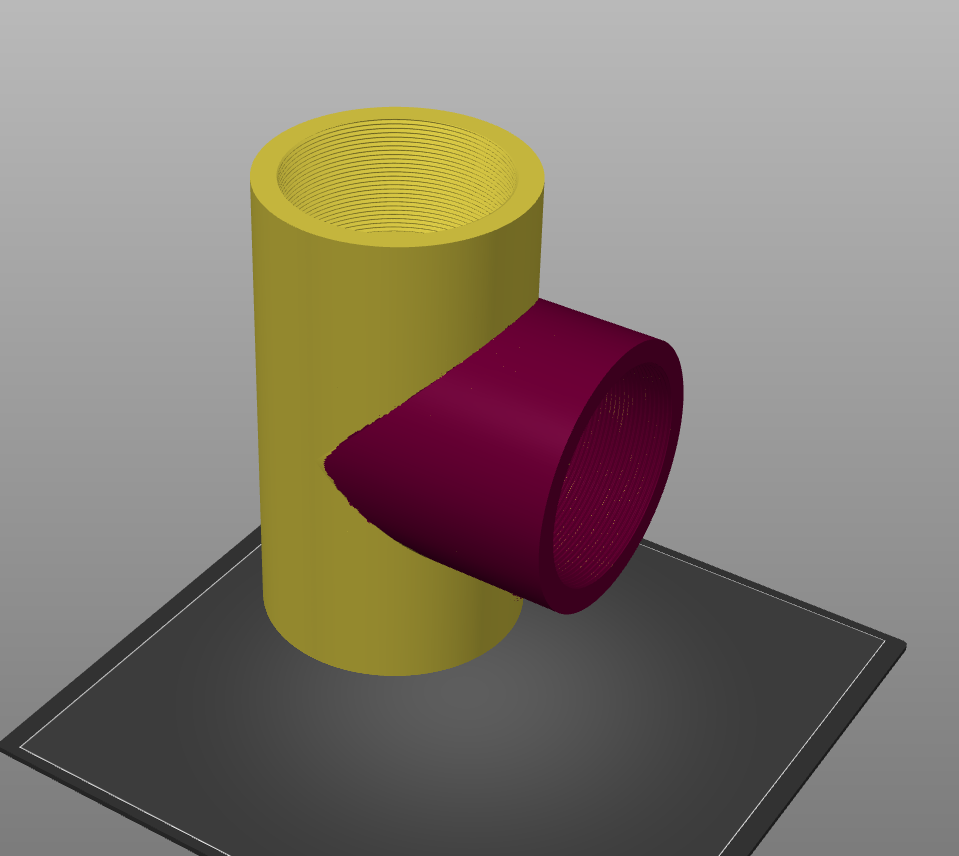
\includegraphics[width=0.5\textwidth]{t_pipe}
	\ccaption{T-Rohr als LMD-druckbarer Teil}{Eigener Screenshot PrusaSlicer 2.6.0}
	\label{img:t_pipe}
\end{figure}
\end{document}
